%! Author = nico
%! Date = 17.06.22
\documentclass[a4paper, landscape, 8pt]{scrartcl}
\usepackage{csquotes}
\usepackage{color}
\usepackage{subfiles}

% import template
% use german language
\usepackage[T1]{fontenc}
\usepackage[utf8]{inputenc}
\usepackage[english, ngerman]{babel}
\usepackage{lmodern}

% format
\usepackage{geometry}
\geometry{top=1.2cm, left=0.4cm, right=0.4cm}
\textheight = 550pt

% author
\usepackage{authblk}

% tables / tabular
\usepackage{tabularx}
\usepackage{makecell}

% math
\usepackage{amsmath}
\usepackage{amssymb}
\usepackage{amsfonts}
\usepackage{enumitem}

% graphic
\usepackage{graphicx}

% multi column
\usepackage{multicol}

%compact items
\setlist{topsep=0pt, leftmargin=4mm, nolistsep}
\setlength{\parindent}{0cm}

% header and footer
\usepackage{fancyhdr}
\pagestyle{fancy}

% header
\fancyhead[RO]{\AUTHOR | \INSTITUTE}
\fancyhead[LO]{\TITLE}

% footer
\fancyfoot[RO]{\CREATED}

\renewcommand\headrulewidth{0pt}
\renewcommand\footrulewidth{0pt}
\headsep = 2pt
\footskip = 0pt

% define Section format
\usepackage{sectsty}
\usepackage{titlesec}
\usepackage[dvipsnames]{xcolor}

\titleformat{name=\section}[block]{\sffamily\normalsize}{}{0pt}{\colorsection}
\titlespacing*{\section}{0pt}{0pt}{0pt}
\newcommand{\colorsection}[1]{%
	\colorbox{sectioncolor!80}{\parbox{0.98\linewidth}{\vspace{-1pt}\color{white}\ #1 \vspace{-2pt}}}}

% define Subsection format
\titleformat{name=\subsection}[block]{\sffamily\small}{}{0pt}{\colorsubsection}
\titlespacing*{\subsection}{0pt}{0pt}{0pt}
\newcommand{\colorsubsection}[1]{%
	\colorbox{subsectioncolor!80}{\parbox{0.98\linewidth}{\vspace{-1pt}\color{white}\ #1 \vspace{-2pt}}}}

% define SubSubsection format
\titleformat{name=\subsubsection}[block]{\sffamily\small}{}{0pt}{\colorsubsubsection}
\titlespacing*{\subsubsection}{0pt}{0pt}{0pt}
\newcommand{\colorsubsubsection}[1]{%
	\colorbox{subsubsectioncolor!60}{\parbox{0.98\linewidth}{\vspace{-1pt}\color{white}\ #1 \vspace{-2pt}}}}


% define colors
\definecolor{sectioncolor}{HTML}{191919}
\definecolor{subsectioncolor}{HTML}{8c195f}
\definecolor{subsubsectioncolor}{HTML}{d72864}

\definecolor{b}{RGB}{0, 115, 192 } %Default highlight color
\definecolor{p}{RGB}{0, 43, 54} %Dark page color
\definecolor{t}{RGB}{131, 148, 150} %Dark text color

\definecolor{darkgreen}{RGB}{0,150,0}
\definecolor{dkgreen}{rgb}{0,0.6,0}
\definecolor{gray}{rgb}{0.5,0.5,0.5}
\definecolor{mauve}{rgb}{0.58,0,0.82}
\definecolor{DarkPurple}{rgb}{0.4, 0.1, 0.4}
\definecolor{DarkCyan}{rgb}{0.0, 0.5, 0.4}
\definecolor{LightLime}{rgb}{0.3, 0.5, 0.4}
\definecolor{Blue}{rgb}{0.0, 0.0, 1.0}
\definecolor{h}{RGB}{1, 101, 163}

% code listings
\usepackage{listings}
\usepackage{color}
\usepackage{beramono}
\usepackage{hyperref}
\hypersetup{
    colorlinks,
    linkcolor={black},
    citecolor={blue!50!black},
    urlcolor={blue!80!black}
}

\definecolor{bluekeywords}{rgb}{0,0,1}
\definecolor{greencomments}{rgb}{0,0.5,0}
\definecolor{redstrings}{rgb}{0.64,0.08,0.08}
\definecolor{xmlcomments}{rgb}{0.5,0.5,0.5}
\definecolor{types}{rgb}{0.17,0.57,0.68}

\definecolor{lstborder}{RGB}{149, 73, 119}
\definecolor{lstbackground}{RGB}{242, 232, 239}

\definecolor{lightgray}{rgb}{.9,.9,.9}
\definecolor{darkgray}{rgb}{.4,.4,.4}
\definecolor{purple}{rgb}{0.65, 0.12, 0.82}

\lstdefinelanguage{JavaScript}{
	keywords={typeof, new, true, false, catch, function, return, null, catch, switch, var, if, in, while, do, else, case, break},
	keywordstyle=\color{blue}\bfseries,
	ndkeywords={class, export, boolean, throw, implements, import, this},
	ndkeywordstyle=\color{darkgray}\bfseries,
	identifierstyle=\color{black},
	sensitive=false,
	comment=[l]{//},
	morecomment=[s]{/*}{*/},
	commentstyle=\color{purple}\ttfamily,
	stringstyle=\color{red}\ttfamily,
	morestring=[b]',
	morestring=[b]"
}

\lstdefinestyle{eclipse-style}{
	frame=single,
	rulecolor=\color{lstborder},
	backgroundcolor=\color{lstbackground},
	language=C,
	showstringspaces=false,
	basicstyle=\ttfamily\scriptsize,
	keywordstyle=\color{RoyalBlue}\ttfamily,
    stringstyle=\color{darkgreen}\ttfamily,
	commentstyle=\color{DarkPurple!60}\ttfamily,
	identifierstyle=\color{black}\ttfamily,
	escapeinside={£}{£}, % latex scope within code
	breaklines=true,
	breakatwhitespace=true,
	showspaces=false,
	showtabs=false,
	tabsize=2,
	morekeywords={length},
	numberstyle=\tiny\color{black},
	aboveskip = 0em,
	belowskip = 0em,
	xleftmargin= 0em,
	framexleftmargin= 0em,
	gobble=20
}
\lstset{
	style=eclipse-style
	% literate=  % Allow for German characters in lstlistings.
	% {Ö}{{\"O}}1
	% {Ä}{{\"A}}1
	% {Ü}{{\"U}}1
	% {ü}{{\"u}}1
	% {ä}{{\"a}}1
	% {ö}{{\"o}}1}
}

% creation date
\usepackage{filemod}
\newcommand{\CREATED}{\filemodprintdate{\jobname}}

% front page
\newcommand{\AUTHOR}{Nico Fehr }
\newcommand{\INSTITUTE}{Ostschweizer Fachhochschule}

% no indentation
\setlength{\parindent}{0cm}

% new item tabitem for bullet points in tables
\newcommand{\tabitem}{~~\llap{\textbullet}~~}

% document information
\newcommand{\SUBJECT}{}
\newcommand{\TITLE}{Cheat Sheet für WE1 (Web Engineering 1)}

% document content
\begin{document}

    \begin{multicols*}{4}
        \setlength{\columnseprule}{0pt}
        \footnotesize

        \section{Architektur Webanwendung}
        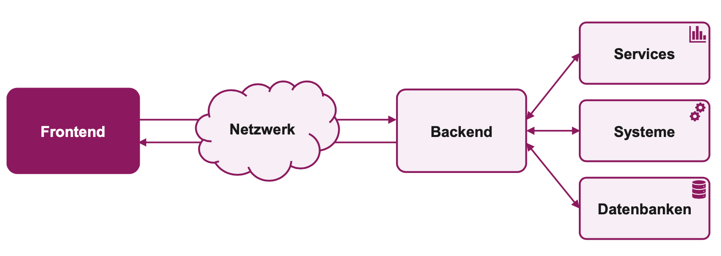
\includegraphics[width=\columnwidth]{graphic/32-architektur-webanwendung}

        \section{HTML}
        \begin{itemize}
            \item doctype
            \item \textbf{html} Root-Element
            \subitem z.B. Sprache (für Übersetzer / Screen-Reader)
            \item \textbf{head} Metadaten
            \subitem Nur 1 head-Element
            \subitem Daten über das Dokument
            \subitem werden nicht dargestellt
            \item \textbf{body} Sichtbarer Inhalt der Webseite
            \subitem nur 1 body-Element
        \end{itemize}

        \begin{lstlisting}[language=HTML]
                    <!DOCTYPE html>
                    <html lang="en">
                        <head>
                            <meta charset="UTF-8">
                            <link rel="icon"href="ost-favicon-32x32.png">
                            <title>hello</title>
                        </head>
                        <body>
                            <!--this is a comment-->
                            <h1>Hello World</h1>
                            <input type="password" value="1234">
                        </body>
                    </html>
        \end{lstlisting}

        \begin{itemize}
            \item Auszeichnungssprache / Markup Language
            \item beschreibt \textbf{Struktur} eines Dokuments
            \item Trennung \textbf{Inhalt} und \textbf{Darstellung}
        \end{itemize}
        \textcolor{subsectioncolor}{HyperText Markup Language} \\
        \begin{tabularx}{\columnwidth}{l | X}
            \textbf{Hypertext} & Verlinkung von Dokumenten möglich \\
            \textbf{Markup} & Semantische Auszeichnung von Inhalten \texttt{(h1, p, footer, \ldots)} \\
            \textbf{Language} & Definierte Syntax und Bedeutung
        \end{tabularx}

        \begin{itemize}
            \item HTML-Dateien werden decodiert, in DOM übersetzt und vom Browser gerendert
            \item HTML-Code prüfen $\to$ W3C-Validator
        \end{itemize}

        \subsection{Metadaten}
        \begin{lstlisting}[language=HTML]
                    <head>
                        <meta charset="UTF-8"> <title>Title</title>
                        <link rel="stylesheet" href="styles.css">
                        <link rel="icon" href="ost-favicon32x32.png">
                        <meta name="author" content="name, frieder.loch@ost.ch">
                        <meta name="viewport" content="width=device-width, initial-scale=1">
                        <meta name="description" content="A description of the page">
                        <meta name="robots" content="index" />
                    </head>
        \end{lstlisting}

        \subsubsection{Kategorien}
        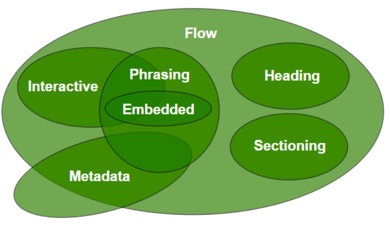
\includegraphics[scale=0.3]{graphic/00-categories-elements}

        \subsubsection{Elemente mit Kategorie und Semantik}
        \begin{tabularx}{\columnwidth}{l | X}
            \textbf{Element} & \textbf{Semantik} \\
            \hline
            \texttt{<h1> - <h6>} & Überschriften; h1 höchste Stufe\\
            \hline
            \texttt{<p>} & Absatz\\
            \hline
            \texttt{<blockquote>} & Zitat\\
            \hline
            \texttt{<br>} & Semantischer Umbruch\\
            \hline
            \texttt{<b>} & \enquote{Bring Attention To}: Wichtig für User\\
            \hline
            \texttt{<code>} & Programm-Code\\
            \hline
            \texttt{<img>} & Bild\\
            \hline
            \texttt{<em>} & Hervorhebung anzeigen\\
            \hline
            \texttt{<strong>} & Starke hervorhebung anzeigen\\
            \hline
            \texttt{<mark>} & Relevanz indizieren\\
            \hline
            \texttt{<cite>} & Name eines Werks, Buch markieren\\
            \hline.
            \texttt{<dfn>} & Definition eines Begriffs markieren
        \end{tabularx}

        \subsubsection{Seitenstruktur mit semantischen Elementen}
        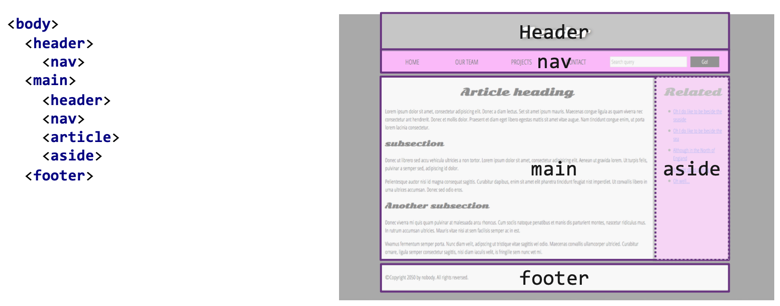
\includegraphics[scale=0.25]{graphic/26-seitenstruktur-semantisch}

        \subsubsection{Semantisch / Nicht-Semantisch}
        Semantik: Zuordnung von Bedeutung zu Texten \\
        \begin{tabularx}{\columnwidth}{l | X}
            Schlecht: "div-Soup" & \textbf{Besser}: semantisches HTML \\
            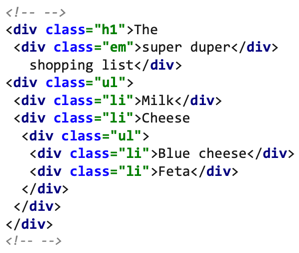
\includegraphics[scale=0.3]{graphic/01-div-soup} &
            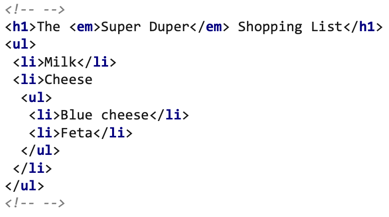
\includegraphics[scale=0.25]{graphic/02-semantic-html}
        \end{tabularx}

        \subsubsection{\texttt{article}-Element}
        In sich geschlossener Abschnitt eines Dokuments, Seite oder Anwendung die unabhängig verteilt oder wiederverwendbar sein soll. \\
        \begin{lstlisting}[language=HTML]
                    <article>
                        <header>
                            <h2>Jurassic Park</h2>
                        </header>
                        <section>
                            <p>Way too scary for me.</p>
                            <footer>
                                <p>Posted on <time datetime="2020-01-01 00:01">January 1</time> by Lisa.</p>
                            </footer>
                        </section>
                        <!-- -->
                        <footer>
                            <p>Posted on <time datetime="2021-01-16 19:00">January 16</time> by Staff.</p>
                        </footer>
                    </article>
        \end{lstlisting}

        \subsubsection{\texttt{section}-Eelement}
        Allgemeine Unterteilung des Dokuments, z.B. thematische Gruppierung des Inhalts mit Überschrift. \\
        $\to$ weniger unabhängig als \texttt{article} \\
        \begin{lstlisting}[language=HTML]
                    <main>
                        <h1>Star Wars</h1>
                        <section>
                            <!-- Inhalte -->
                        </section>
                        <section id="user-reviews">
                            <article>
                                <!-- Inhalt des Artikels -->
                            </article>
                            <article>
                                <!-- Inhalt des Artikels -->
                            </article>
                        </section>
                    </main>
        \end{lstlisting}
        \subsubsection{\texttt{figure}-Element}
        \begin{lstlisting}[language=HTML]
                    <figure>
                        <img src="/media/cc0-images/elephant.jpg" alt="Elephant at sunset">
                        <figcaption>An elephant at sunset</figcaption>
                    </figure>
        \end{lstlisting}

        \subsection{Auswahl des richtigen Elements}
        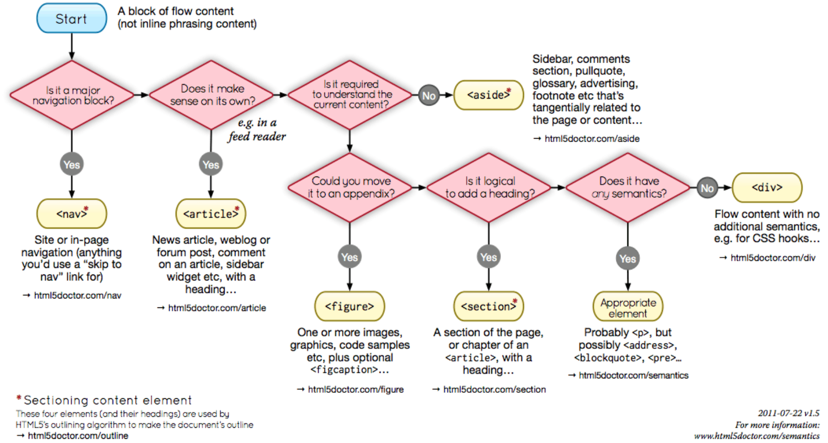
\includegraphics[width=\columnwidth]{graphic/27-auswahl-element}

        \subsection{\textbf{Mögliche Fragen}}
        \begin{itemize}
            \item Wieso sollte ich semantisches HTML verwenden?
            \subitem \textbf{Leichtere Entwicklung:} erhalten einige Funktionen kostenlos, verständlicheres Markup
            \subitem \textbf{Mobile-Freundlich:} Geringere Dateigrösse, leichter responsive zu machen
            \subitem \textbf{SEO:} Suchmaschinen gewichten Schlüsselwörter in Überschriften, Links, \ldots höher
            \subitem \textbf{Zugänglich:} Semantisches Markup ist mit Screenreader deutlich einfacher zu verwenden
            \item Wie kann ich eine gegebene Webseite mit semantischen HTML auszeichnen?
            \subitem mit Tags: nav, article, figure, aside, section
            \item Wo ist Tag Omission möglich?
            \subitem img (must not have end tag)
            \subitem p (start tag required)
            \subitem html
            \subitem input (must not have end tag)
        \end{itemize}

        \section{CSS}
        \begin{itemize}
            \item Inhalt von Darstellung trennen
            \item Unterschiedliche Styles für unterschiedliche Ausgabemedien
            \item Styles auf Elementgruppen anwenden
            \item Regel besteht aus Selektoren und Deklarationsblock
        \end{itemize}

        \subsection{Syntax}
        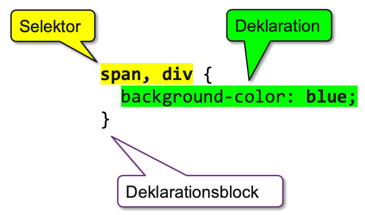
\includegraphics[scale=0.2]{graphic/28-css-syntax}

        \subsection{CSS-Datei in HTML laden}
        \begin{lstlisting}[language=HTMl]
                    <link rel="stylesheet" href="file.css" />
        \end{lstlisting}
        
        \subsection{Selektoren}
        Selektoren sind Case-Sensitiv! (id und class Attribute klein schreiben, zusammengesetzte Worte: kebab-case) \\
        \begin{tabularx}{\columnwidth}{l X}
            Typ & Selektiert \textbf{alle} Elemente vom angegeben Typ \\
            \hline
            ID & Selektiert \textbf{alle} Elemente mit angegebener ID \\
            \hline
            Klassen & Styling ähnlicher Elemente
            \begin{itemize}
                \item \texttt{.recent}: Elemente mit dieser Klasse
                \item \texttt{.recent.explicit}: Elemente mit beiden Klassen
                \item \texttt{article.recent}: article-Elemente mit Klasse recent
            \end{itemize}
            \textbf{Tipp:} Semantische Klassennamen wählen
        \end{tabularx}

        \subsubsection{Pseudo-Elemente}
        Styling von \textbf{bestimmten Teilen} von selektierten Elementen
        \begin{tabularx}{\columnwidth}{X}
            \textbf{Element} \\
            \texttt{::first-line} \\
            \texttt{::after / ::before}\\
            \texttt{::selection}
        \end{tabularx}
        
        \subsubsection{Pseudo-Klassen}
        \begin{tabularx}{\columnwidth}{X X}
            \textbf{Selektor-Typ} & \textbf{Beispiel} \\
            \hline
            \texttt{:nth-child()} & {\bfseries \texttt{span:nth-child(1) span:nth-child(odd) span:nth-child(event)}} \\
            \hline
            \texttt{:first-child} & {\bfseries \texttt{span:first-child}} \\
            \hline
            \texttt{:last-child} & {\bfseries \texttt{span:last-child}} \\
            \hline
            \texttt{:hover} & \\
            \hline
            \texttt{:visited} & \\
            \hline
            \texttt{:active / :focus} &
        \end{tabularx}

        \begin{multicols*}{3}
            \begin{lstlisting}
                    .recent
                        span
                        span <-- nth-child
                        span
            \end{lstlisting}

            \columnbreak

            \begin{lstlisting}
                    .recent
                        span <-- first-child
                        span
                        span
            \end{lstlisting}

            \columnbreak

            \begin{lstlisting}
                    .recent
                        span
                        span
                        span <-- last-child
            \end{lstlisting}
        \end{multicols*}


        \subsubsection{Kombinatoren}
        \begin{tabularx}{\columnwidth}{X X}
            \textbf{Selektor-Typ} & \textbf{Beispiel} \\
            \hline
            Nachfahren (decendant) & \texttt{.recent div} \\
            \hline
            \textbf{Direkte} Nachfahren (child) & \texttt{.recent > div} \\
            \hline
            Angrenzende Geschwister (\textbf{next} siblings) & \texttt{.recent > p:first-of-type + p} \\
            \hline
            Alle Geschwister (\textbf{subsequent} siblings) & \texttt{.recent > p:first-of-type ~ p} \\
        \end{tabularx}

        \begin{multicols*}{2}
            \begin{lstlisting}
                    .recent
                        div         <-- decendant
                            div     <-- decendant
            \end{lstlisting}

            \begin{lstlisting}
                    .recent
                        div         <-- child
                            div
            \end{lstlisting}

            \columnbreak

            \begin{lstlisting}
                    .recent
                        p
                        p   <-- +-Selector
                        p
                        p
            \end{lstlisting}

            \begin{lstlisting}
                    .recent
                        p
                        p   <-- ~-Selector
                        p   <--
                        p   <--
            \end{lstlisting}
        \end{multicols*}
        
        \subsection{Kaskade}
        \begin{itemize}
            \item Mehrere Deklarationen betreffen 1 Element
            \item Kaskade löst Konflikte auf
            \item Kaskade betrachtet folgende Komponenten:
            \subitem Woher kommt Style?
            \subitem Spezifität des Selektors
            \subitem Reihenfolge der Styles
            \subitem \texttt{!important}
        \end{itemize}
        Priorität:
        \begin{enumerate}
            \item Autor:in (Externe / Interne / Inline Styles)
            \item Benutzer:in (Browser-Einstellungen)
            \item Browser (Default-Werte zur Darstellung)
        \end{enumerate}

        \begin{itemize}
            \item Innerhalb der Punkte: Sortieren nach Spezifität
            \item Bei gleicher Spezifität: \textbf{Später} deklarierte Eigenschaft gewinnt
            \item \texttt{!important}-Deklarationen der Benutzer:in gewinnen immer
        \end{itemize}

        \subsubsection{Spezifität}
        \begin{itemize}
            \item Regeln werden nach Spezifität gewichtet
            \item Vier Zähler (A, B, C, D) mit Startwert 0
            \subitem \textbf{\texttt{a++}} Inline-Styles
            \subitem \textbf{\texttt{b++}} ID-Selektoren
            \subitem \textbf{\texttt{c++}} Klassen-Selektoren, Pseudoklassen (: \ldots) und Attribute ([\ldots])
            \subitem \textbf{\texttt{d++}} Typ-Selektoren und Pseudoelemente (:: \ldots)
            \item Bei gleicher Spezifität: Reihenfolge
        \end{itemize}

        \begin{tabular}{|l|c|c|c|c|l|}
            \hline
            Selektor & a & b & c & d & = \\
            \hline
            h1 & 0 & 0 & 0 & 1 & 0001 \\
            \hline
            ul li & 0 & 0 & 0 & 2 & 0002 \\
            \hline
            \#identifier & 0 & 1 & 0 & 0 & 0100 \\
            \hline
            h1\#identifier & 0 & 1 & 0 & 1 & 0101 \\
            \hline
            style=\enquote & 1 & 0 & 0 & 0 & 1000 \\
            \hline
            p:first-child & 0 & 0 & 1 & 1 & 0011 \\
            \hline
            \#editor p & 0 & 1 & 0 & 1 & 0101 \\
            \hline
        \end{tabular}

        \begin{itemize}
            \item Universalselektor "\texttt{*}" wird ignoriert
            \item Pseudoklasse \texttt{:not()} wird ignoriert (Selektoren innerhalb Klammern nicht)
         \end{itemize}

        \subsection{Box Model}
        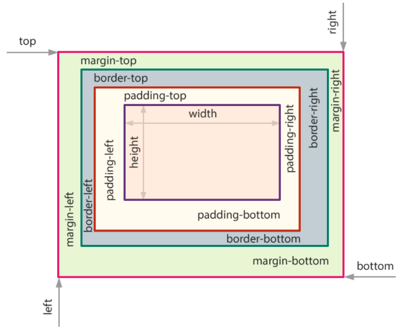
\includegraphics[scale=0.34]{graphic/03-box-model}
        \\
        Element besteht aus:
        \begin{itemize}
            \item Content: Inhalt
            \item Padding: Innenabstand
            \item Border: Rahmen
            \item Margin: Aussenabstand
        \end{itemize}

        \section{Usability}
        \subsection{Heuristiken}
        \textbf{Heuristik:} Sammlung von erprobten \enquote{Daumenregeln}
        \begin{itemize}
            \item Sicherheitsabfragen
            \item Möglichkeit zum Undo bereitstellen
            \item Klare, unterscheidbare Beschriftungen
            \item Unterschiedliches sollte unterschiedlich sein
        \end{itemize}

        \subsection{Wahrnehmung}
        \textbf{Aufmerksamkeit} kann \textbf{gelenkt} werden

        \subsubsection{Change Blindness}
        \begin{itemize}
            \item Veränderungen, die in einem Bereich auftreten, der vom Aufmerksamkeitsfokus entfernt ist, werden eher übersehen
            \item Passiert wenn visuelles Signal für Änderung fehlt
            \item Aufmerksamkeit auf Änderungen lenken
        \end{itemize}

        \subsubsection{Lesen}
        \enquote{Web Users don't read, they scan} \\
        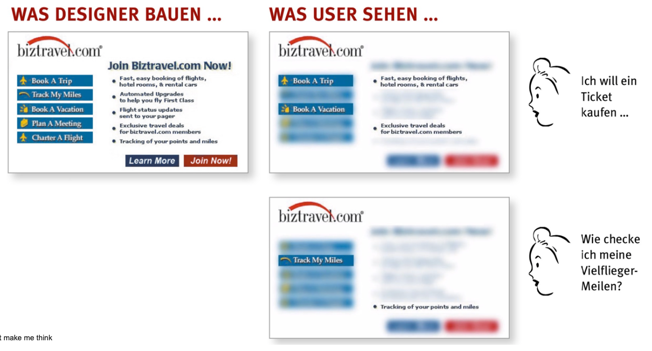
\includegraphics[scale=0.3]{graphic/10-users-read} \\
        Augenführung durch:
        \begin{itemize}
            \item Grafiken
            \item Textgrössen
            \item Farben
        \end{itemize}

        $\to$ Informationen \textbf{\textcolor{subsectioncolor}{hierarchisch}} darstellen \\
        Methoden zur Strukturierung \\
        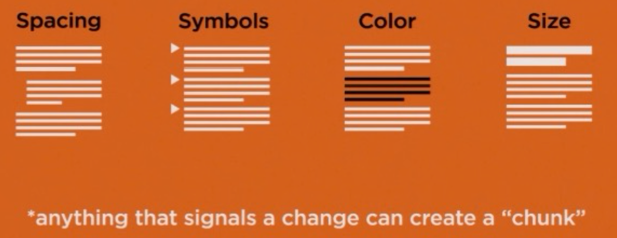
\includegraphics[scale=0.2]{graphic/12-strukturierung}

        \subsubsection{Unterstützen verschiedener Rezeptionsformen}
        \begin{tabularx}{\columnwidth}{l | l}
            \textbf{Rezeption} & \textbf{Gestaltung} \\
            \hline
            Scannen & Akzente \\
            & \tabitem Überschriften \\
            & \tabitem Schlüsselwörter, -bilder \\
            & \tabitem Links / Suchhilfen \\
            \hline
            Skimmen & Zusammenfassen \\
            & \tabitem kurze Absätze \\
            & \tabitem Listen / Tabellen \\
            & \tabitem Info-Grafik \\
            \hline
            Lesen & Details \\
            & \tabitem Längere Seiten mit Fliesstext \\
            & \tabitem Format zum Ausdrucken
        \end{tabularx}

        \subsubsection{Sehfähigkeit}
        \begin{itemize}
            \item Auge hat kleinen \enquote{Scharfen Fleck} (\textit{Fovea})
            \item Statische Informationen im peripheren Bereich werden leicht übersehen
        \end{itemize}
        \begin{tabularx}{\columnwidth}{l | X}
            Bereich & Was wird wahrgenommen? \\
            \hline
            \textcolor{subsectioncolor}{zentraler Bereich} &
            Farben und Details \\

            \textcolor{subsectioncolor}{peripherer Bereich} &
            Bewegungen und Veränderungen
        \end{tabularx}
        
        \subsection{Affordance von UI-Elementen}
        
\includegraphics[scale=0.23]{graphic/09-push-flip-rotate}
        \\
        \textbf{Affordance:} Natürlich wahrnehmbare Nutzungsmöglichkeit eines Geräts \\

        Affordances ermöglichen:
        \begin{itemize}
            \item Konventionen befolgen
            \item Konsistente Verwendung
            \item Beschriftung beschreibt Aktion
            \item Metaphern mit Vorsicht verwenden
        \end{itemize}

        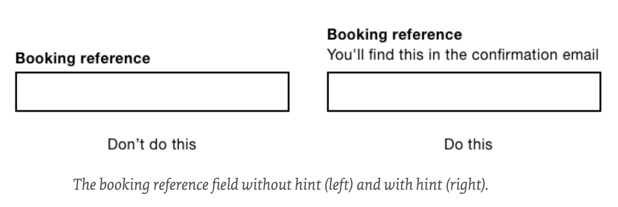
\includegraphics[scale=0.2]{graphic/13-affordance-booking-reference} \\
        Gute Beschriftungen mit entsprechenden Hinweisen

        \begin{tabularx}{\columnwidth}{l | X}
            \textcolor{subsectioncolor}{Gibson} &
            Natürlich wahrnehmbare Nutzungsmöglichkeit eines Geräts \\

            \hline
            \textcolor{subsectioncolor}{Norman} &
            \makecell[l]{
                \textit{Wahrgenommene} affordance \\
                Touchscreen $\to$ Tap, Swipe, \ldots \\
                Maus $\to$ Clicken, Draggen, \ldots
            }
        \end{tabularx}

        \subsection{10 Nielsen Usability Heuristiken}
        \begin{enumerate}[label=\color{subsectioncolor}\theenumi]
            \item Sichtbarkeit des Systemstatus
            \item Übereinstimmung zwischen System und realer Welt
            \subitem Bekannte Begriffe verwenden (Sprache der User)
            \subitem Konventionen respektieren
            \item Freiheit und Kontrolle der User
            \item Konsistenz und Standards
            \subitem Begriffe konsistent verwenden
            \subitem Links unterstreichen, Buttons klickbar
            \item Fehlervermeidung
            \subitem Undo $\to$ behebt Fehler beim Experimentieren
            \subitem Genügend grosse \enquote{Touch-Targets}
            \subitem Vorzeitige Evaluation von Datumsfeldern
            \item Wiedererkennen statt erinnern
            \item Flexibilität und effiziente Nutzung
            \item Ästhetik und minimalistische Gestaltung
            \item Hilfe beim Erkennen und Beheben von Fehlern
            \item Hilfe und Dokumentation
        \end{enumerate}

        \subsubsection{Sichtbarkeit des Systemstatus}
        Zustand des Systems zeigen \\
        Zeigt Möglichkeiten der Interaktion
        \begin{itemize}
            \item Welche \textit{Objekte} können selektiert werden
            \item Welche \textit{Aktionen} können ausgeführt werden
            \item Welche \textit{Navigationsmöglichkeiten} existieren
        \end{itemize}

        \subsection{Visuelle Gestaltung {\tiny Gestaltungsgesetze}}
        \begin{itemize}
            \item Beeinflusst lesbarkeit
            \item Lenkt Aufmerksamkeit
            \item Schafft Vertrauen und Glaubwürdigkeit
            \item Stärkt die Marke
        \end{itemize}

        \subsubsection{Gesetze der Zusammengehörigkeit}
        Welche Elemente werden als zusammengehörig wahrgenommen? \\
        
\includegraphics[width=\columnwidth]{graphic/11-usability-zusammen}

        \subsubsection{Gesetz der Ähnlichkeit}
        \begin{itemize}
            \item Elemente die ähnlich aussehen werden als Gruppe interpretiert
            \item Ähnliches Zusammenfassen
            \subitem Farben, Grössen, Bewegungen, Formen
            \item Strukturierung stärker
            \subitem Grad der Ähnlichkeit der Elemente
            \subitem Kontrast zu benachbarten Elementen
            \subitem Anzahl der ähnlichen Eigenschaften
        \end{itemize}

        \subsubsection{Gesetz der Nähe}
        \begin{itemize}
            \item Elemente die \textbf{räumlich} nah beieinander liegen, werden als Gruppe interpretiert
            \item Benachbarte Elemente gruppieren (Spalten / Zeilen)
            \item Benachbarte Elemente sollten zusammengehören
            \item Abständen bewusst werden
        \end{itemize}

        \subsection{Farben}

        \begin{multicols*}{2}
            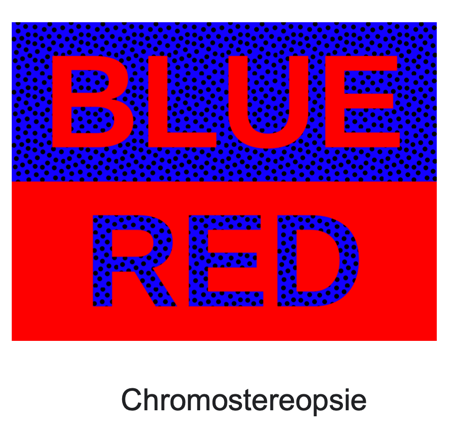
\includegraphics[scale=0.15]{graphic/14-chromostereopsie}

            \begin{itemize}
                \item Wenige Farben (< 6, besser 2 + 1)
                \item Standards / Normen (z.B. Styleguides)
                \item Kulturelle Aspekte !
                \item Ausreichender Kontrast
                \item \textbf{Pyhisologische Aspekte}
                \subitem Farbfehlsichtigkeit
                \subitem Schlechte Farbkombis
                \subitem Seheinschränkungen beachten
            \end{itemize}
        \end{multicols*}

        \subsubsection{Kulturelle Aspekte}
        \textcolor{red}{Rot} nicht immer \enquote{Stop / Achtung} \\
        \textcolor{green}{Grün} nicht immer \enquote{Gut / Weiter}

        \subsubsection{Farbfehlsichtigkeit}
        9\% aller Männer, 0.8\% aller Frauen haben Rot-Grün Sehschwäche

        \subsection{Usability Testing}
        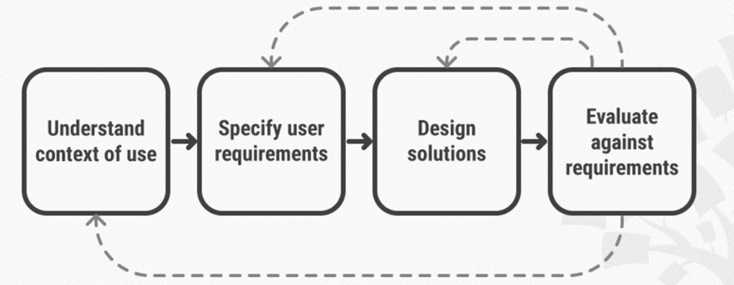
\includegraphics[width=\columnwidth, height=40pt]{graphic/15-usability-testflow}
        \begin{itemize}
            \item Probleme erkennen
            \item Verbesserungsmöglichkeiten identifizieren
            \item User kennenlernen
        \end{itemize}

        \subsubsection{Flow of Information}
        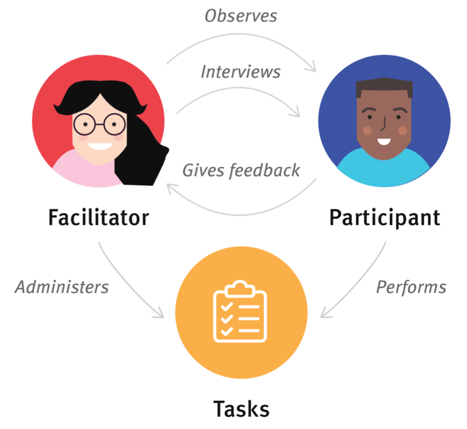
\includegraphics[scale=0.24]{graphic/16-usability-flow-information}
        
        \subsubsection{Iterative Entwicklung}
        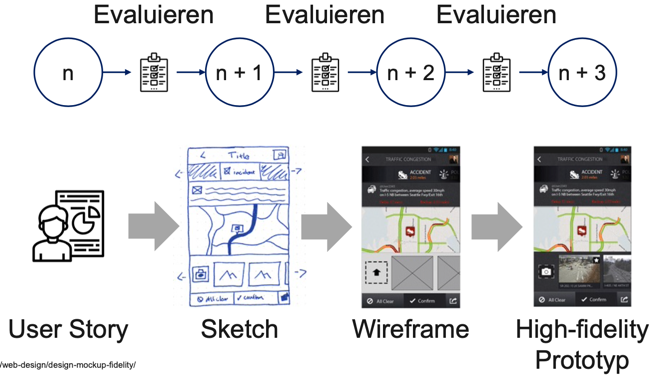
\includegraphics[width=\columnwidth]{graphic/17-iterative-entwicklung}

        \section{DOM}
        \subsection{DOM-Lifecycle}
        \subsubsection{Ladezustand des Dokuments}
        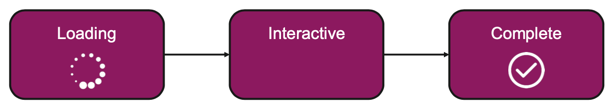
\includegraphics[scale=0.22]{graphic/04-ladezustand-dom}
        \begin{enumerate}
            \item \texttt{Loading}
            \subitem Dokument lädt noch
            \item \texttt{Interactive}
            \subitem Dokument geladen/geparst
            \subitem Ressourcen (Scripts, Bilder / Video, Stylesheets) werden noch geladen
            \subitem \textbf{Event:} \textcolor{darkgreen}{DOMContentLoaded}
            \item \texttt{Complete}
            \subitem Dokument und Ressourcen geladen
            \subitem \textbf{Event:} \textcolor{darkgreen}{load}
        \end{enumerate}

        \subsubsection{\texttt{async / defer}}
        \begin{tabularx}{\columnwidth}{l X}
            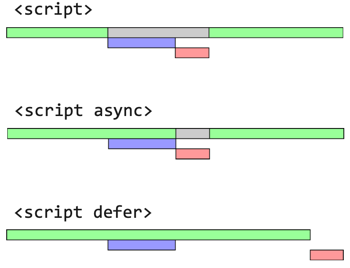
\includegraphics[scale=0.25]{graphic/29-async-defer-loading-times} & 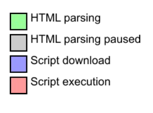
\includegraphics[scale=0.4]{graphic/30-async-defer-legend}
        \end{tabularx}

        \subsection{DOM-Interfaces}
        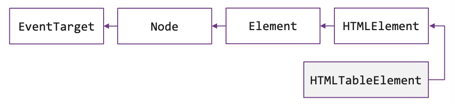
\includegraphics[scale=0.35]{graphic/31-dom-interfaces} \\
        Knoten im DOM-Tree implementieren Interfaces \\
        \begin{tabularx}{\columnwidth}{l | X}
            \texttt{EventTarget} & Wichtige Methoden \\
            & \tabitem \texttt{addEventListener} \\
            & \tabitem \texttt{removeEventListener} \\
            & \tabitem \texttt{dispatchEvent} \\
            & Objekt kann Events empfangen \\
            \hline
            \texttt{Node} & \tabitem Einheitliches Interface für Tree \\
            & \tabitem z.B. finden und Traversieren der Nodes \\
            & Wichtige Properties \\
            & \tabitem \texttt{childNodes} \\
            & \tabitem \texttt{firstChild} \\
            & \tabitem \texttt{nextSibling} \\
            & Wichtige Methoden \\
            & \tabitem \texttt{appendChild()} \\
            & \tabitem \texttt{removeChild()} \\
            \hline
            \texttt{Element} & \tabitem Basis für Elemente im DOM-Tree \\
            & \tabitem Definiert Methoden auf Element-Level \\
            & Wichtige Properties \\
            & \tabitem \texttt{id} \\
            & \tabitem \texttt{className / classList} \\
            & \tabitem \texttt{innerHTML} \\
            & Wichtige Methoden \\
            & \tabitem \texttt{getAttribute()/setAttribute()/ toggleAttribute()} \\
            & \tabitem \texttt{closest()} \\
            \hline
            \texttt{HTMLElement} & Repräsentiert HTML-Element \\
            & Wichtige Properties \\
            & \tabitem \texttt{dataset} \\
            & \tabitem \texttt{style} \\
            & \tabitem \texttt{hidden} \\
            \hline
            \texttt{HTMLTableElement} & Methoden um mit Tabelle umzugehen \\
            & Wichtige Methoden \\
            & \tabitem \texttt{createCaption()} \\
            & \tabitem \texttt{createTFoot()} \\
            & \tabitem \texttt{createTHead()}
        \end{tabularx}
        
        \subsection{DOM-Navigation {\tiny Element \texttt{Node}}}
        Node besitzt Eigenschaften zur Navigation im DOM
        \begin{itemize}
            \item .parentElement
            \item .childNodes
            \item .children
            \item .firstChild
            \item .firstElementChild
            \item .nextSibling
            \item .nextElementSibling
        \end{itemize}
        \textbf{HTML-Elemente sind auch Knoten} \\
        \texttt{document.querySelector("\#progress-div").parentElement;}

        \subsection{\texttt{window}}
        \begin{itemize}
            \item Fenster, in dem das Dokument dargestellt wird
            \item Stellt globale Objekte zur Verfügung
            \subitem \texttt{console}
            \subitem \texttt{document}
            \subitem \texttt{HTMLDocument}
            \item Globale Variablen liegen auf \texttt{window}
        \end{itemize}
        
        \subsection{DOM-Selektion}
        {\small\texttt{getElementBy}}
        \begin{itemize}
            \item \texttt{document.getElementById (<idString>)}
            \item \texttt{document.getElementByName (<nameString>) // Form-Element}
            \item \texttt{<searchRootElement>.getElementsByClassName (<singleClassString>) // HTMLCollectionOf<Element>}
            \item \texttt{<searchRootElement>.getElementsByTagName (<tagString>)}
        \end{itemize}

        {\small\texttt{querySelector}}
        \begin{itemize}
            \item \texttt{<searchRootElement>.querySelector (<selectorString>) // first match}
            \item \texttt{<searchRootElement>.querySelectorAll (<selectorString>) // NodeListOf<HTMLElement>}
            \item \texttt{<searchRootElement>.closest (<selectorString>) // first matching ancestor}
            \item \texttt{<searchRootElement>.matches (<selectorString>) // boolean}
        \end{itemize}


        \subsection{DOM-Manipulation}
        \subsubsection{createElement \& appendChild}
        \begin{itemize}
            \item Schneller bei kleinen Änderungen
            \item DOM-Referenzen bleiben erhalten
            \item Event-Handler bleiben erhalten
        \end{itemize}
        \begin{lstlisting}[language=JavaScript]
                    // 1
                    const newEl = document.createElement('div');
                    newEl.appendChild(document.createTextNode('Hello'));
                    document.querySelector("#container").appendChild(newEl);

                    // 2
                    const newEl2 = document.createElement('div');
                    newEl2.innerText = 'World';
                    document.querySelector("#container").appendChild(newEl2)
        \end{lstlisting}

        \subsubsection{createDocumentFragment}
        \begin{lstlisting}[language=JavaScript]
                    const fragment = document.createDocumentFragment();
                    parent.appendChild(fragment);
        \end{lstlisting}

        \subsubsection{innerHTML}
        \begin{itemize}
            \item Wahrscheinlich schneller als createElement
            \item Code ist lesbarer
        \end{itemize}
        \begin{lstlisting}[language=JavaScript]
                    // Inhalt schreiben
                    const c = document.querySelector("#container");
                    c.innerHTML = '<div>Changed</div>';
                    c.innerHTML = `<div>${content}</div>`;

                    // Inhalt loeschen
                    c.innerHTML = '';

                    // An bestimmter Position einfuegen
                    insertAdajcentHTML(position, text)
        \end{lstlisting}

        \subsubsection{Umgang mit CSS-Klassen}
        \begin{itemize}
            \item <element>.className
            \item Klassen als String, getrennt mit Space
            \item <element>.classList
            \item Klassen als DOMTokenList
            \item DOMTokenList bietet Hilfsfunktionen
            \item add / remove / toggle / contains / replace
        \end{itemize}

        \subsubsection{DOM Attribute}
        \begin{itemize}
            \item setAttribute('attributeName', 'newAttributeValue')
            \item setzt beliebige Werte beliebiger Attribute
            \item setzt auch entsprechende Property
            \item removeAttribute('attributeName')
            \item Löscht Attribut
        \end{itemize}

        \subsection{DOM-Events}
        \begin{tabularx}{\columnwidth}{l}
            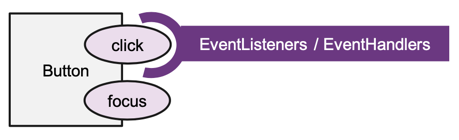
\includegraphics[scale=0.35]{graphic/06-dom-event-listener} \\
            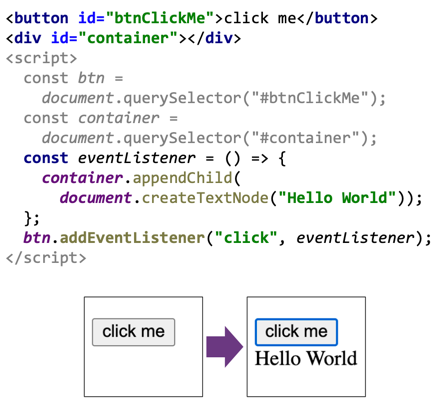
\includegraphics[scale=0.35]{graphic/07-click-me-example}
        \end{tabularx}
        \begin{itemize}
            \item \texttt{HTMLElement} bietet Events, auf die \texttt{EventListener} registriert werden können
            \item Mit \texttt{addEventListener} werden \texttt{EventListener} registriert
            \item \texttt{EventListener} wird beim Eintreten des Events aufgerufen
        \end{itemize}
        
        \subsubsection{addEventListener}
        {\small\texttt{target.addEventListener(type, listener[, options])}}
        \\
        Type
        \begin{itemize}
            \item Name vom Event
        \end{itemize}
        Listener
        \begin{itemize}
            \item \texttt{EventListener} Funktion
            \item Inline oder separat definiert
        \end{itemize}
        Options-Objekt
        \begin{itemize}
            \item \texttt{capture:} \> Reagiert auf Events in der Capture-Phase (\texttt{boolean})
            \item \texttt{once:} \> Listener wird automatisch nach erster Aktivierung entfernt (\texttt{boolean})
            \item \texttt{passive:} \> Für Performance-Optimierungen (\texttt{boolean})
        \end{itemize}

        \subsubsection{EventListener registrieren}
        \begin{lstlisting}[language=JavaScript]
                    document.querySelector("#1").addEventListener("click", () => alert('1')); // 1

                    document.querySelector("#2").onclick = () => alert('2'); // 2

                    <button onclick="alert('3')">3</button> // 3
        \end{lstlisting}

        \subsubsection{Event-Objekt}
        Folgende Properties \& Methoden
        \begin{itemize}
            \item target
            \subitem Element von dem Event ausging
            \item currentTarget
            \subitem Zeigt auf Element, das Event-Listener registriert hat
            \item preventDefault()
            \subitem Verhindert Default-Aktionen
            \item stopPropagation()
            \subitem Event von Bubbling/Capturing abhalten
        \end{itemize}
        Spezifische Typen
        \begin{itemize}
            \item MouseEvent
            \item WheelEvent
            \item InputEvent
        \end{itemize}

        \subsubsection{KeyboardEvent-Objekt}
        EventListener erhält Event-Objekt mit weitern Infos
        \begin{itemize}
            \item change: Was wurde geändert?
            \item keydown: Welche Taste gedrückt?
            \item ctrlKey: War Control Taste gedrückt?
        \end{itemize}
        \begin{lstlisting}[language=JavaScript]
                    document.querySelector("input").addEventListener("keydown", (event) => {
                        console.log(event.key);
                    })
        \end{lstlisting}

        \subsubsection{Event-Bubbling}
        \begin{itemize}
            \item Event-Handler in Parent Element definieren
            \item click-Events aller Children in bubble-Phase bearbeiten
            \item Nur ein Handler nötig, unabhängig von Anzahl der Bilder
        \end{itemize}
        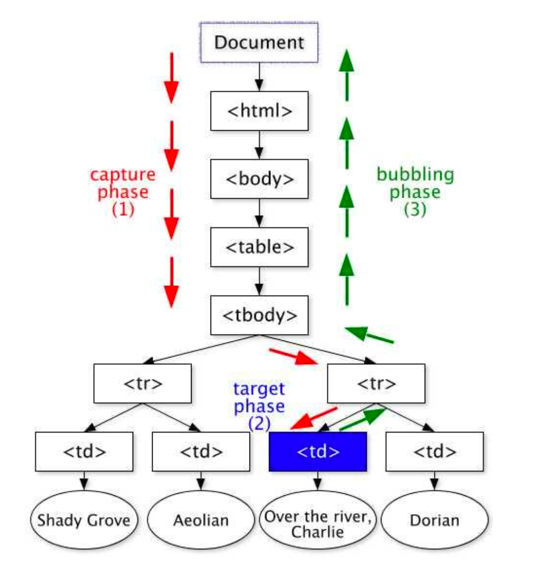
\includegraphics[scale=0.3]{graphic/08-event-bubbling}
        \begin{enumerate}
            \item Capture-Phase
            \subitem Event durchläuft DOM-Tree von Wurzel zum Blatt
            \subitem Jedes Element kann reagieren (muss aber nicht)
            \item Target-Phase
            \subitem Event wird auf Target ausgelöst
            \item Bubble-Phase
            \subitem Event durchläuft DOM-Tree vom Blatt zur Wurzel
            \subitem Jedes Element kann reagieren (muss aber nicht)
            \subitem Nicht jedes Event durchläuft Bubble-Phase
        \end{enumerate}

        \section{HTTP, REST, AJAX}

        \subsection{HTTP}
        \begin{itemize}
            \item Anfordern von Ressourcen über Netzwerk
            \item \textbf{Client} und \textbf{Server} tauschen \textbf{Nachrichten} (Request / Response) aus
            \item Nachrichten bestehen aus \textbf{Header} und \textbf{Body}
            \item \textbf{Request:} Client $\to$ Server
            \subitem \textbf{Typ:} GET, POST, PUT, DELETE, PATCH
            \subitem Headers
            \item \textbf{Response:} Server $\to$ Client
            \subitem \textbf{Status Code:} 404, 200, \ldots
            \subitem Body
        \end{itemize}

        \subsubsection{Request}
        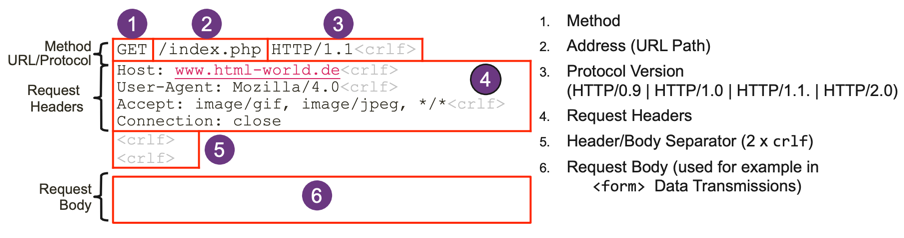
\includegraphics[width=\columnwidth]{graphic/36-http-request}

        \subsubsection{Response}
        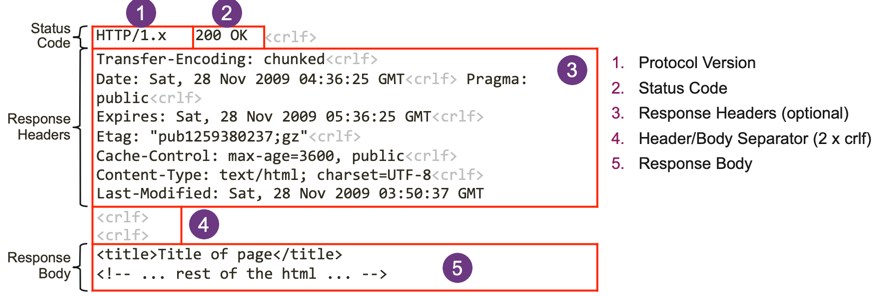
\includegraphics[width=\columnwidth]{graphic/37-http-response}

        \subsubsection{Response Status Codes}
        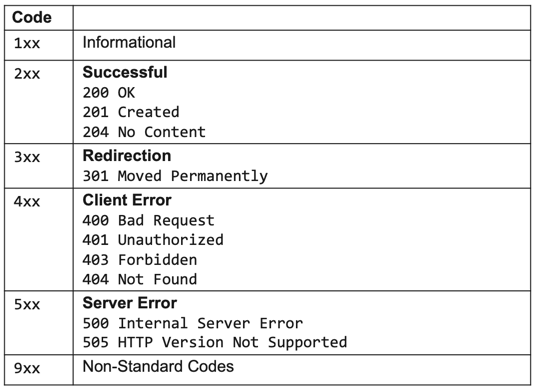
\includegraphics[width=\columnwidth]{graphic/38-http-status-codes}

        \subsubsection{Request $\to$ Response}
        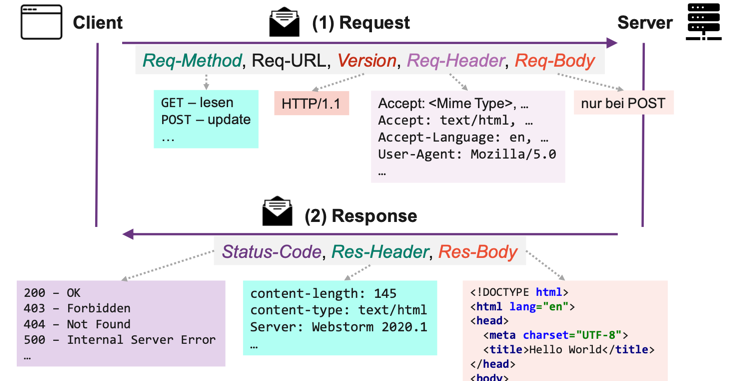
\includegraphics[width=\columnwidth]{graphic/20-request-response}

        \subsubsection{Request-Methoden}
        \begin{tabularx}{\columnwidth}{l | X}
            \textbf{GET} & Daten abrufen, soll keine Seiteneffekte haben \\
            \hline
            \textbf{POST} & Sendet Daten an Server, erzeugt meist neue Ressource (nicht-idempotent) \\
            \hline
            \textbf{PUT} & Ersetzt alle Darstellungen der Zielressource durch hochgeladenen Inhalt (idempotent) \\
            \hline
            \textbf{DELETE} & Entfernt alle Darstellungen der durch URI angegebenen Zielressource
        \end{tabularx}

        \subsubsection{Request absetzten JS}
        \begin{lstlisting}[language=JavaScript]
                    async function fetchFromURL() {
                      try {
                        const response = await fetch('result.json', { method: 'GET'});
                        if(response.ok) {
                          const content = await response.text();
                          console.log(content);
                        }
                      } catch(e) {
                        // Fehlerbehandlung
                      }
                    }
        \end{lstlisting}

        \subsection{Node.js}

        \subsubsection{HTML-Server}
        \begin{lstlisting}[language=JavaScript]
                    function requestHandler(req, res) {
                        if (req.url === '/favicon.ico') {...}
                        const parsedURL = new URL(req.url, `http://${req.headers.host}`);
                        const responseHtml = createResponseHtml(parsedURL);

                        res.setHeader('Content-Type', 'text/html');
                        res.statusCode = (responseHtml) ? 200 : 404;
                            res.end(responseHtml);
                    }
                    function createResponseHtml(parsedURL) {
                        if (parsedURL.pathname === '/hello') {
                            return `<h1>Hello</h1> <p>${parsedURL.href}</p>`;
                        }
                        return '';
                    }
        \end{lstlisting}

        \subsubsection{HTML File Server mit node-static}
        \begin{lstlisting}[language=JavaScript]
                    import http from 'http';
                    import nstatic from 'node-static';

                    const PORT = 8080;
                    const fileServer = new nstatic.Server('./pub');

                    function requestHandler(req, res) {
                        fileServer.serve(req, res);
                    }

                    const server = http.createServer(requestHandler);
                    server.listen(PORT, () => console.log('Node listening on Port ', PORT));
        \end{lstlisting}


        \subsection{Promises}
        \enquote{A sign, or a \textcolor{subsectioncolor}{reason for hope that something may happen}, especially something good.} \\
        \textbf{Promise-Objekt} stellt möglichen Abschluss (oder Misserfolg) einer asynchronen Operation und den daraus resultierenden Wert dar. \\
        Die \textbf{asynchrone Methode} gibt ein Versprechen (Promise) zurück, den Wert \textbf{in der Zukunft} zu liefern

        \subsubsection{Daten von URL laden}
        \begin{lstlisting}[language=JavaScript]
                    async function fetchFromURL() {
                        return new Promise ((resolve, reject) => {
                            const response = fetch('https://stone.sifs0005.infs.ch/ranking')
                                .then(res => res.json())
                                .then(json => resolve(json))
                        }).catch(
                            err => reject(err)
                        );
                    }
        \end{lstlisting}

        \subsubsection{Anwendung in JavaScript}
        Promise kapselt \texttt{async}-Operation

        \begin{itemize}
            \item \textbf{\textcolor{subsectioncolor}{pending:}} Operation aktiv
            \item \textbf{\textcolor{subsectioncolor}{fulfilled:}} Operation erfolgreich beendet und Ergebnis verfügbar (Settled)
            \item \textbf{\textcolor{subsectioncolor}{rejected:}} Operation gescheitert (Settled)
        \end{itemize}

        Möglichkeit auf Zustandsänderungen zu reagieren
        \begin{itemize}
            \item \texttt{.then(..)}
            \item \texttt{.catch(..)}
            \item \texttt{.finally(..)}
        \end{itemize}

        \subsubsection{Konstruktor}
        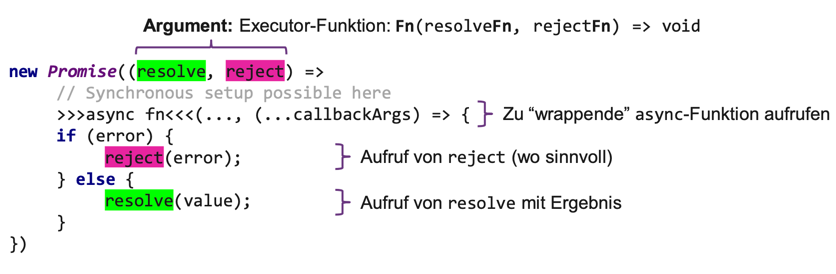
\includegraphics[width=\columnwidth]{graphic/21-promise-constructor}

        \subsubsection{Promises - Lifecycle}
        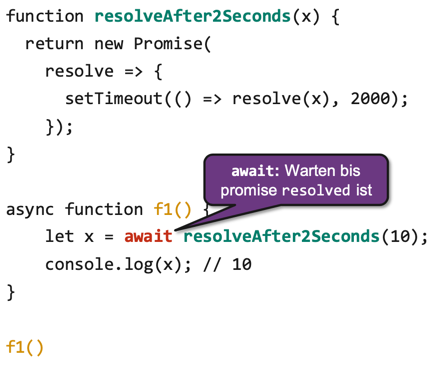
\includegraphics[scale=0.3]{graphic/22-await-promises}

        \subsubsection{\texttt{await} und \texttt{then} {\tiny Async Songs Demo}}
        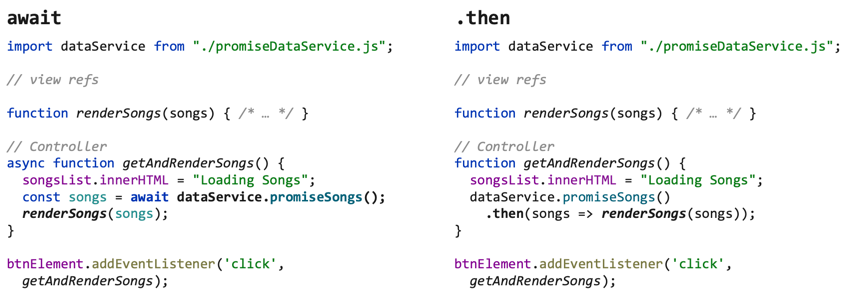
\includegraphics[width=\columnwidth]{graphic/23-async-songs-demo}

        \subsection{Fetch}

        \subsubsection{Doppeltes \texttt{then} oder \texttt{await}}
        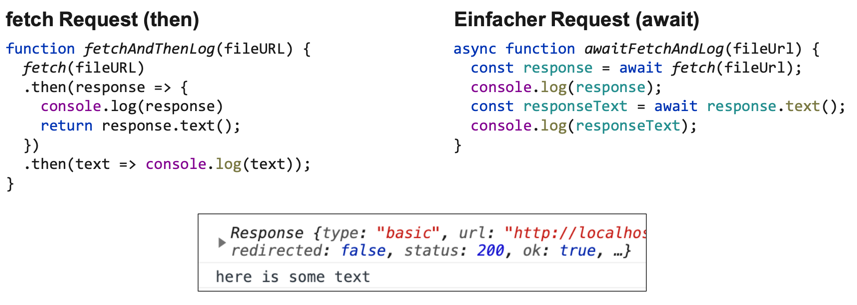
\includegraphics[width=\columnwidth]{graphic/24-double-await-or-then}

        \subsubsection{Einfacher Request}
        \texttt{const \textcolor{darkgreen}{myTextFetchPromise} = fetch('./01b-someText.txt');} \\
        \begin{tabularx}{\columnwidth}{| X | X |}
            \hline
            \texttt{\textcolor{darkgreen}{myTextFetchPromise}} & \texttt{-> Promise \{<fulfilled>: Response\}} \\
            \hline
            \texttt{\textcolor{red}{response} = \textcolor{blue}{await} \textcolor{darkgreen}{myTextFetchPromise};} & \texttt{-> Promise \{type: "basic", ...\}} \\
            \hline
            \texttt{\textcolor{orange}{p2} = \textcolor{red}{response}.text();} & \texttt{-> Promise \{<pending>\}} \\
            \hline
            \texttt{\textcolor{orange}{p2}} & \texttt{-> fulfilled} \\
            \hline
            \texttt{text = \textcolor{blue}{await} \textcolor{orange}{p2};} & \texttt{-> "here is some text"} \\
            \hline
        \end{tabularx}

        \subsection{REST}
        \subsubsection{Webservice}
        \enquote{Webservice is a software system designed to support interoperable machine-to-machine interaction over a network} \\
        \textbf{Ziel}
        \begin{itemize}
            \item Dienst (Service) nach aussen zur Verfügung stellen
            \item Andere Geräte können Webservice über Netzwerk (Web) nutzen
        \end{itemize}

        \subsubsection{Richardson's Maturity Model}
        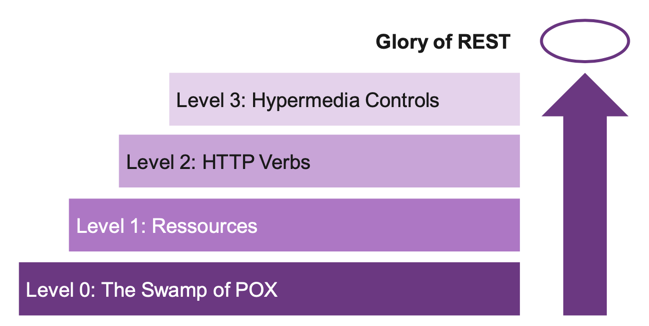
\includegraphics[scale=0.25]{graphic/25-richardsons-maturity-model}
        
        \begin{tabularx}{\columnwidth}{X}
            \hline
            \textbf{Level 0: The Swamp of POX} \\
            Server hat nur einen Endpunkt \\
            $\to$ nur POST \\
            \hline
            \textbf{Level 1: Ressources} \\
            $\to$ Server hat mehrere Endpunkte \\
            $\to$ Jeder Endpunkt ist unterschiedlicher Request \\
            \hline
            \textbf{Level 2: HTTP verbs} \\
            GET / POST / DELETE / PUT / PATCH \\
            $\to$ z.B GET um Dinge zu holen und POST um Dinge zu speichern \\
            $\to$ PUT ersetzen einer Ressource \\
            $\to$ GET keine Seiteneffekte \\
            $\to$ POST hat Seiteneffekte \\
            \hline
            \textbf{Level 3: Hypermedia Controls} \\
            $\to$ Client wird gesagt was mit Ressource gemacht werden muss \\
            $\to$ z.B. Buchung eines Termins ist über andere Ressource möglich \\
            \hline
        \end{tabularx}

        \subsubsection{Resource-oriented Architecture}
        \begin{itemize}
            \item Ressource
            \subitem Alles was wichtig genug ist um eigenständig referenziert zu werden
            \item Name
            \subitem Eindeutige ID der Ressource (z.B. URI)
            \item Repräsentation
            \subitem Ressourcen haben mehrere Repräsentationen
            \item Links
            \subitem Hyperlinks verknüpfen Ressourcen
            \item Interface
            \subitem Uniform Interface
            \subitem Benutze Standard \texttt{http}-Verben
            \item Statuslos Kommunikation
        \end{itemize}

        \subsubsection{Ressource Name}
        \begin{itemize}
            \item Ressourcen mit URI identifizieren
            \item Jede Ressource hat eindeutigen URI
            \subitem \texttt{orders/1}
            \subitem \texttt{books/0-330-25864-8}
            \item Sub-Ressourcen
            \subitem Wenn Sub-Ressource ohne Parent nicht existieren kann (\textbf{Komposition})
            \subitem \texttt{customers/1/orders}
            \subitem \texttt{topics/1/comments}
        \end{itemize}
        
        \subsubsection{Hypermedia As The Engine Of Application State {\tiny(HATEOAS)}}
        \begin{itemize}
            \item Prozessgedanke in Ressource
            \item Media-Typen beschreiben Ressource
            \item Aktionen werden ausgeführt beim Folgen von Links
            \item Jede Antwort beinhaltet Application State
            \item Selbstbeschreibende APIs erzeugen Flexibilität
        \end{itemize}
        
        \subsubsection{REST vs. Remote Procedure Call (RPC)}
        \begin{itemize}
            \item REST stellt Ressource in den Mittelpunkt
            \item RPC stellt einzelne Operationen in den Vordergrund
        \end{itemize}

        \subsubsection{POST example}
        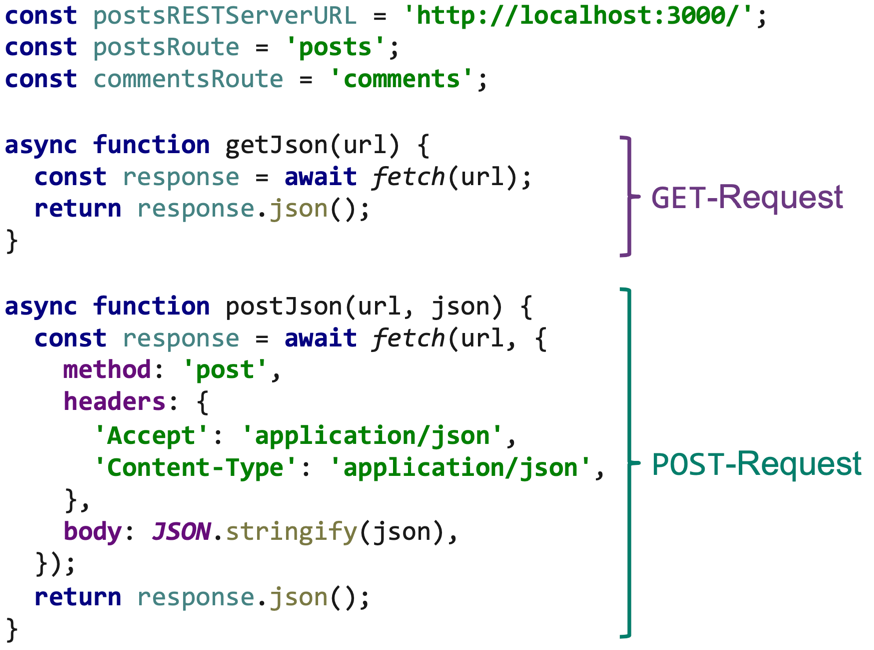
\includegraphics[width=\columnwidth]{graphic/41-post-example}

        \subsection{AJAX}
        Asynchronous JavaScript and XML \\
        with AJAX, web applications can send data to and retrieve from a server asynchronously (in the background) without interfering with the display and behaviour of the existing page.

        \begin{itemize}
            \item Asynchrone Anfrage and Server (blockiert nicht Event-Loop)
            \item Inkrementelle Updates statt kompletter Reload
            \item Keine Seitenwechsel (Single Page App)
            \item Datenformat heute meist JSON (statt XML)
        \end{itemize}

        \subsubsection{Vorteile}
        \begin{itemize}
            \item Flüssigere Interaktion
            \item Seite ohne Neuladen aktualisieren
            \item Kürzere Zeit bis zum First Meaningful Point, da Daten nach Bedarf geladen werden
            \item In Formularen wird Cursor nicht aus aktuellen Feld genommen
        \end{itemize}

        \subsubsection{Nachteile {\tiny bei Single-Page Apps}}
        \begin{itemize}
            \item Zurück-Funktion und URLs müssen separat programmiert werden (History-API)
            \item Darstellung und Verwaltung von Loading Indicators
        \end{itemize}

        \subsubsection{Mehrfachversuche}
        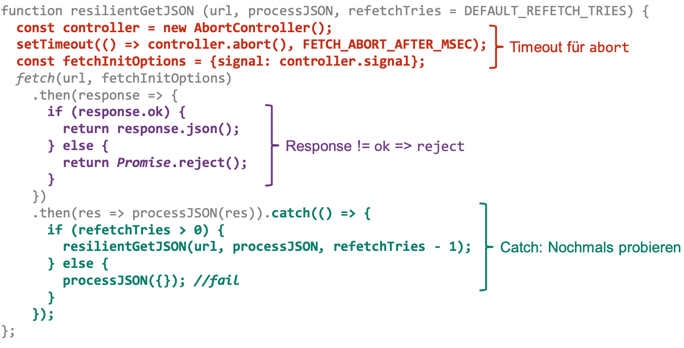
\includegraphics[width=\columnwidth]{graphic/40-mehrfachversuche}

        \subsubsection{Abortable Fetch}
        \begin{lstlisting}[language=JavaScript]
                    async function fetchWithTimeout(resource, options = {}) {
                        const timeout = 8000;
                        const controller = new AbortController();
                        const id = setTimeout(() => controller.abort(), timeout);
                        try {
                            const response = await fetch(resource, {signal: controller.signal});
                            if (response.status === 200) {
                                return response.json();
                            } else {
                                return response;
                            }
                        } catch (error) {
                            throw error;
                        } finally {
                            clearTimeout(id);
                        }
                    }
        \end{lstlisting}

        \subsubsection{Polling}
        \begin{lstlisting}[language=JavaScript]
                    async function updateChatFromServer () {
                        messages = await dataService.getChat(chatId); updateView();
                    }
                    async function joinChat (event) {
                        event.preventDefault();
                        try {
                            joinError = false;
                            messages = await dataService.addToChat(chatId, `${handle} joined chat`); state = STATE_CHATTING;
                            setInterval(updateChatFromServer, 10000);
                        } catch {
                            joinError = true;
                        }
                        updateView();
                    }
                    joinChatForm.addEventListener('submit', joinChat);
        \end{lstlisting}

        \section{Clean Code}
        \subsection{Namen Beispiel}
        \begin{itemize}
            \item Schlechtester Name für Variable?
            \subitem \textcolor{subsectioncolor}{data}
            \item Zweitschlechtester Name?
            \subitem \textcolor{subsectioncolor}{data2}
            \item Drittschlechtester Name?
            \subitem \textcolor{subsectioncolor}{data\_2}
        \end{itemize}

        \subsection{Namensgebung}
        \begin{itemize}
            \item Funktionen $\to$ Verben
            \item Klassen $\to$ Substantive (Nomen)
        \end{itemize}

        \enquote{A name must be \textit{short, intuitive, descriptive}} \\
        \texttt{const \textbf{a} = 5;} \> vs. \> \texttt{const \textbf{postCount} = 5;} \\

        Namen sollten \textbf{aussprechbar} sein \\
        \texttt{const \textbf{cDOB} = 0;} \> vs. \> \texttt{const \textbf{clientDateOfBirth} = 0;} \\

        \begin{itemize}
            \item Bekannte Wörter
            \item Spezifische Namen
            \item Konsistenz (Project Glossary)
            \item Kontext muss nicht wiederholt werden
            \item Namen auf passender Abstraktionsebene
        \end{itemize}
        
        \subsection{Funktionen}
        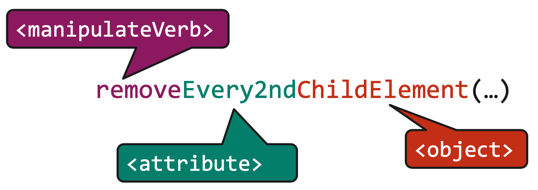
\includegraphics[scale=0.20]{graphic/18-name-funktionen}

        Funktionen sollten\ldots
        \begin{itemize}[label=...]
            \item \textbf{kurz} sein
            \item \textbf{eine} Aufgabe erledigen
            \item \textbf{möglichst wenig Argumente} haben
            \item einen \textbf{beschreibenden Namen} haben und \textbf{nur das tun}
        \end{itemize}

        \subsection{AirBnB Styleguide {\tiny Regeln}}
        \begin{tabularx}{\columnwidth}{l | X}
            \texttt{no-var} & var nicht verwenden\\
            \hline
            \texttt{prefer-const} & let nur für Variablen mit dynamischer Zuordnung\\
            \hline
            \texttt{quotes} & Strings immer mit single-quotes\\
            \hline
            \texttt{no-param-reassign} & Parameter nicht in Funktion ändern (auch nicht Parameter-Properties)\\
            \hline
            \texttt{operator-linebreak} & Kein Linebreak direkt vor oder nach Zuweisung (=)\\
            \hline
            \texttt{eqeqeq} & === und !== nutzen (nicht ==, !=)\\
            \hline
            \texttt{space-infix-ops} & nicht const x = y + 5\\
            \hline
            \texttt{eol-last} & Am Ende des Files ein Return\\
            \hline
            \texttt{no-multiple-empty-lines} & nur 1 Leerzeile\\
            \hline
            \texttt{semi} & Zeilen sollten mit Semikolon abgeschlossen werden\\
        \end{tabularx}

        \subsection{Linting}
        \begin{itemize}
            \item Statische Quellcodeanalyse
            \item Prüfung gegen hinterlegten Regelsatz
            \item Unterstützt bei Behebung von Regelverstössen
            \item Verbessert Codequalität \& Codierungsstil
        \end{itemize}

        \subsubsection{While-Schleifen nicht verwenden}
        \begin{tabularx}{\columnwidth}{X}
            \texttt{'@web-and-design/wed/no-while': 'warn',} \\
            \hline
            \texttt{for (var i = 0; i < xs.length; i++) \{} \\
            \texttt{console.log(xs[i]);} \\
            \texttt{\}} \\
            \hline
            \texttt{xs.forEach((x, i) => console.log(x))}
        \end{tabularx}

        \subsubsection{Kein switch/if else für Aktionen}
        \begin{tabularx}{\columnwidth}{X}
            \texttt{'@web-and-design/wed/use-action-map': 'warn',} \\
            \hline
            \texttt{const evalLookup = \{scissors: \{ scissors: 0, stone: 1, paper: -1, \}, ...\};} \\
            \texttt{evalLookup[playerHand][systemHand];} \\
            \hline
            \texttt{function getGameEval(playerHand, systemHand) \{} \\
            \texttt{ return evalLookup[playerHand][systemHand];} \\
            \texttt{\}}
        \end{tabularx}

        \subsection{MVC {\tiny Model-View-Controller}}
        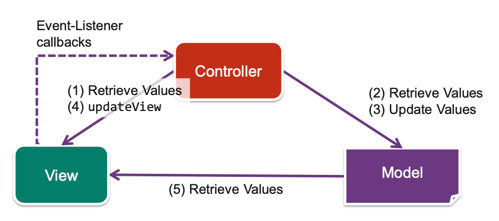
\includegraphics[scale=0.3]{graphic/33-mvc}
        \begin{itemize}
            \item Model
            \subitem Datenmodell
            \subitem App Zustand
            \subitem User Daten
            \subitem Logik
            \subitem \textit{Keine View Refs}
            \item View
            \subitem Anzeige
            \item Controller
            \subitem User Eingaben
            \subitem View-Wechsel (Routing)
        \end{itemize}

        \section{JavaScript}
        \begin{lstlisting}[language=HTML]
                    <!-- type=module -> ESM wird aktiviert -->
                    <head>
                        <title>Test</title>
                        <script src="index.js" type="module"></script>
                    </head>
        \end{lstlisting}

        \subsection{Typeof}
        \begin{tabular}{l | l}
            Undefined & 'undefined' \\
            Null & 'object' \\
            Boolean & 'boolean' \\
            Number & 'number' \\
            BigInt (EcmaScript 2020) & bigint' \\
            String value & 'string' \\
            Function & 'function \\
            Symbol (ECMAScript 6) & 'symbol' \\
            All other & 'object'
        \end{tabular}

        \subsection{Falsy / Thruthy}
        \begin{tabular}{l | l}
            \textbf{false-Werte} & \textbf{true-Werte} \\
            false & "0" (String) \\
            0 (zero) & "false" (string) \\
            "" (empty string) & [] \\
            null & \{\} \\
            undefined & \\
            NaN &
        \end{tabular}

        \subsection{Number}
        \begin{itemize}
            \item Nach Definition sind alle Zahlen "floats" (Gleitkommazahlen)
            \item Engines versuchen floats auf integers abzubilden - falls möglich
        \end{itemize}
        \textbf{NaN ("Not a Number")}
        \begin{itemize}
            \item Ist ein Error-Wert
            \item 0/0 => NaN
            \item Hat auch den Type "number"
            \item NaN == NaN ist immer false
            \item isNaN() zum überprüfen
        \end{itemize}
        \textbf{Infinity}
        \begin{itemize}
            \item Unendlich
            \item Kann auch negativ sein
        \end{itemize}
        \textbf{Jeder Wert kann in eine Zahl verwandelt werden}
        \begin{itemize}
            \item +(true) == 1
            \item Number(true) == 1
            \item Number(null) == 0
            \item Number(\("\)abc\("\)) => NaN
            \item Ausnahme: Symbol
        \end{itemize}
        \textbf{parseInt( \("\) string \("\) ) | parseFloat( \("\) string \("\) )}
        \begin{itemize}
            \item Parst bis zum ersten Fehler
        \end{itemize}

        \subsection{+ - * / Regeln}
        \begin{itemize}
            \item Punkt vor Strich
            \item Von Links nach Rechts aufgelöst
            \item Spezialfälle
            \subitem String + Value = String
            \subitem Value + String = String
            \item Ansonsten
            \subitem Value (Numerischer Operator) Value = Number
        \end{itemize}

        \subsection{Abstract Equality Comparison Algorithm (==) (===)}
        \begin{lstlisting}[language=JavaScript]
                    console.log([] == false);       //true
                    console.log("" == false);       //true
                    console.log(null == false);     //false
                    console.log(0 == "0");          //true
                    console.log(null == undefined); //true
                    console.log([1,2] == "1,2");    //true
                    console.log(NaN == NaN);        //false
                    console.log([] == ![]);         //true


                    console.log(false === false);   //true
                    console.log(4 === 4);           //true
                    console.log(false === false);   //true
                    console.log([] === false);      //false
                    console.log("" === false);      //false
                    console.log(null === false);    //false
                    console.log(0 === "0");         //false
                    console.log(null === undefined);//false
                    console.log([1,2] === "1,2");   //false
                    console.log(NaN === NaN);       //false
                    console.log([] === ![]);        //false
        \end{lstlisting}

        \subsection{null / undefined}
        
\includegraphics[scale=0.2]{graphic/35-toilet-roll-example}

        \subsection{Array}
        \begin{itemize}
            \item Keine fixe Länge
            \item Index beginnt bei 0
            \item Array bietet Iterator-Methoden an
        \end{itemize}
        
        \subsubsection{.filter()}
        \begin{lstlisting}[language=JavaScript]
                    const words = ['spray', 'limit', 'elite', 'exuberant', 'destruction', 'present'];
                    const result = words.filter(word => word.length > 6);
                    console.log(result);
                    // Expected output: Array ["exuberant", "destruction", "present"]
        \end{lstlisting}

        \subsubsection{.entries()}
        \begin{lstlisting}[language=JavaScript]
                    const array1 = ['a', 'b', 'c'];
                    const iterator1 = array1.entries();
                    console.log(iterator1.next().value);
                    // Expected output: Array [0, "a"]
                    console.log(iterator1.next().value);
                    // Expected output: Array [1, "b"]
        \end{lstlisting}

        \subsubsection{.concat()}
        \begin{lstlisting}[language=JavaScript]
                    const array1 = ['a', 'b', 'c'];
                    const array2 = ['d', 'e', 'f'];
                    const array3 = array1.concat(array2);
                    console.log(array3);
                    // Expected output: Array ["a", "b", "c", "d", "e", "f"]
        \end{lstlisting}

        \subsubsection{.find()}
        \begin{lstlisting}[language=JavaScript]
                    const array1 = [5, 12, 8, 130, 44];
                    const found = array1.find(element => element > 10);
                    console.log(found);
                    // Expected output: 12
        \end{lstlisting}

        \subsubsection{.findIndex()}
        \begin{lstlisting}[language=JavaScript]
                    const array1 = [5, 12, 8, 130, 44];
                    const isLargeNumber = (element) => element > 13;
                    console.log(array1.findIndex(isLargeNumber));
                    // Expected output: 3
        \end{lstlisting}

        \subsubsection{.forEach()}
        \begin{lstlisting}[language=JavaScript]
                    const array1 = ['a', 'b', 'c'];
                    array1.forEach(element => console.log(element));
                    // Expected output: "a"
                    // Expected output: "b"
                    // Expected output: "c"
        \end{lstlisting}

        \subsubsection{.reduce()}
        \begin{lstlisting}[language=JavaScript]
                    const array1 = [1, 2, 3, 4];
                    // 0 + 1 + 2 + 3 + 4
                    const initialValue = 0;
                    const sumWithInitial = array1.reduce(
                      (accumulator, currentValue) => accumulator + currentValue,
                      initialValue
                    );
                    console.log(sumWithInitial);
                    // Expected output: 10
        \end{lstlisting}

        \subsubsection{.map()}
        \begin{lstlisting}[language=JavaScript]
                    const array1 = [1, 4, 9, 16];
                    // Pass a function to map
                    const map1 = array1.map(x => x * 2);
                    console.log(map1);
                    // Expected output: Array [2, 8, 18, 32]
        \end{lstlisting}

        \subsubsection{.some()}
        \begin{lstlisting}[language=JavaScript]
                    const array = [1, 2, 3, 4, 5];
                    // Checks whether an element is even
                    const even = (element) => element % 2 === 0;
                    console.log(array.some(even));
                    // Expected output: true
        \end{lstlisting}

        \subsubsection{.every()}
        \begin{lstlisting}[language=JavaScript]
                    const isBelowThreshold = (currentValue) => currentValue < 40;
                    const array1 = [1, 30, 39, 29, 10, 13];
                    console.log(array1.every(isBelowThreshold));
                    // Expected output: true
        \end{lstlisting}

        \subsubsection{.flat()}
        \begin{lstlisting}[language=JavaScript]
                    const arr1 = [0, 1, 2, [3, 4]];
                    console.log(arr1.flat());
                    // Expected output: Array [0, 1, 2, 3, 4]
                    const arr2 = [0, 1, 2, [[[3, 4]]]];
                    console.log(arr2.flat(2));
                    // Expected output: Array [0, 1, 2, Array [3, 4]]
        \end{lstlisting}

        \subsubsection{.flatMap()}
        \begin{lstlisting}[language=JavaScript]
                    const arr1 = [1, 2, [3], [4, 5], 6, []];
                    const flattened = arr1.flatMap(num => num);
                    console.log(flattened);
                    // Expected output: Array [1, 2, 3, 4, 5, 6]
        \end{lstlisting}

        \subsection{Callback}
        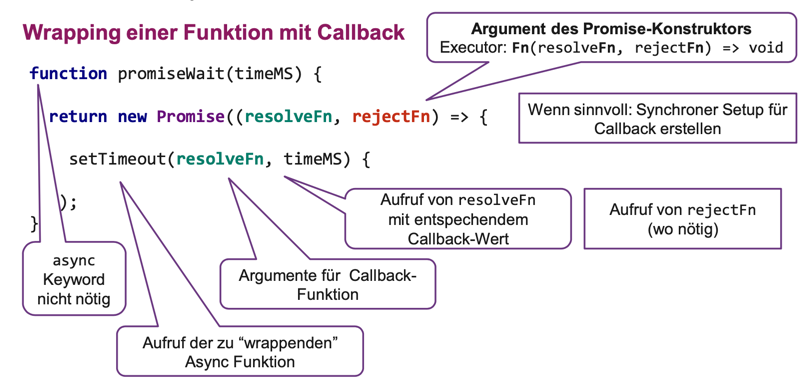
\includegraphics[width=\columnwidth]{graphic/34-wrapping-function-with-callback}

        \subsection{Funktionen}
        \begin{itemize}
            \item Funktionen sind \enquote{First-Class Citizen}
            \subitem können in Variablen gespeichert werden
            \subitem können als Parameter übergeben werden
            \subitem können von Funktionen zurückgegeben werden
            \item Besitzen offene Parameter-Liste
            \subitem mehr oder weniger als deklarierte Anzahl Parameter übergeben werden
            \subitem alle Parameter werden in \texttt{arguments} abgelegt
            \item Funktionen besitzen Properties
            \item Normale Funktion erzeugt eigenen Scope
        \end{itemize}

        \subsubsection{Als Parameter und Rückgabe}
        \begin{lstlisting}[language=JavaScript]
                    function add(a, b){
                        return a + b;
                    }
                    function minus(a, b){
                        return a - b;
                    }
                    function calc(fn, a ,b){
                        console.log(fn(a,b));
                    }

                    calc(add, 3, 4);
                    calc(minus, 3, 4);
        \end{lstlisting}
        \begin{lstlisting}[language=JavaScript]
                    function addTo(a){
                        return function(b){
                            return a + b;
                        }
                    }
                    const addTo3 = addTo(3);
                    addTo3(4);
        \end{lstlisting}
        
        \subsubsection{Offene Parameter-Liste}
        \begin{itemize}
            \item arguments beinhaltet alle Parameter, welche übergeben wurden
            \item arguments ist kein Array
            \subitem \texttt{$\to$ Array.from(arguments)}
        \end{itemize}

        \subsubsection{Properties}
        \begin{itemize}
            \item Funktionen besitzen Properties
            \item .name beinhaltet den Namen der Funktion
            \subitem Anonyme Methoden besitzen keinen "name"
            \subitem Dieser Name wird für den Stacktrace genutzt
            \subitem Falls kein Name angegeben, loggen moderne Browser den Variablenamen
            \item .length beinhaltet Anzahl Parameter der Funktion
        \end{itemize}

        \subsubsection{Rest-Parameters}
        \begin{itemize}
            \item Mit \texttt{...name} kann man letzten Parameter als \enquote{Rest-Parameter} definieren
            \item Parameter wird mit restlichen Werten gefüllt
            \item keine restlichen Parameter erzeugt leeres Array
        \end{itemize}
        \begin{lstlisting}[language=JavaScript]
                    function foo(name, ...params){
                        console.log(1,name);
                        console.log(2,params.join(";"));
                    }
                    foo("Michael", "Gfeller", "OST", "IFS");
        \end{lstlisting}

        \subsubsection{Overloading}
        \begin{itemize}
            \item JavaScript kennt kein \enquote{Function Overloading}
            \item Bei gleichen Funktionsnamen überschreibt die zuletzt definierte die vorhergehenden
            \item Lösung: Interne Wiche (typeof \& arguments) oder sinnvolle default-Werte definieren
        \end{itemize}

        \begin{lstlisting}[language=JavaScript]
                    jQuery.fn.init = function( selector, context ) {
                        //...
                        if ( !selector ) { return this;
                        }
                            // Handle HTML strings
                        if ( typeof selector === "string" ) {
                            //...
                        } else if ( selector.nodeType ) {
                            //...
                        } else if ( jQuery.isFunction( selector ) ) {
                            //...
                        }
                        //...
                        return jQuery.makeArray( selector, this );
                    };
        \end{lstlisting}

        \subsection{Scope}
        \begin{itemize}
            \item Jede Funktion und Objekt generiert einen neuen Scope
            \item Innerhalb von einem Scope kann man auf
            \subitem dessen Variablen
            \subitem gloable Variablen
            \subitem Variablen aller \enquote{Parent}-Scopes zugreifen (Closure, Werte bleiben erhalten)
            \item Ein script-Tag erzeugt keinen Scope
            \item ECMAScript Module erzeugen einen Scope
            \item Global Namespace Pollution
            \subitem Zu viele Variablen und Funktionen im globalen Scope
            \subitem Variablen oder Funktionen mit identischem Namen überschreiben sich
        \end{itemize}

        \begin{lstlisting}[language=JavaScript]
                    const funcA = function(){
                        const a = 1;
                        const funcB = function(){
                            const b = 2;
                            console.log(a, b); // outputs: 1, 2
                        };
                        funcB();
                        console.log(a, b); // Error! b is not defined
                    };
                    funcA();
                    funcB(); // Error! funcB is not defined
        \end{lstlisting}

        \subsection{Strict Mode / 'use strict'}
        \begin{itemize}
            \item Erste Linie in File / Funktion
            \item Strict Mode wird vererbt
            \item Eliminiert \enquote{fails silently}
            \item Falls eine Variable ohne var definiert wird
            \item Falls Read-only werte gesetzt werden (ohne strict: ignoriert)
            \item Eliminiert Probleme wechen es Compiler verunmöglicht Code zu optimieren
            \item Security wird \enquote{leicht} verbessert
            \item Wichtig: Das Laufzeitverhalten ändert sich!
            \item Wichtig: Strict Mode kann nicht mehr entfernt werden
            \item Wichtig: Strict Mode muss pro File aktiviert werden
            \item Wichtig: Strict Mode sollte nicht mit Non Strict Mode zu einem File vereint werden
            \item Immer verwenden ausser Legacy Code, Files werden zusammengefügt
            \item Klasse und ESM sind immer Strict-Mode
        \end{itemize}

        \begin{lstlisting}[language=JavaScript]
                    function a() {
                        a1 = 1; //ok
                    }

                    function c() {
                        'use strict';

                        function b() {
                            b1 = 1; //error
                        }
                        b();
                        a();
                    }
                    c();
        \end{lstlisting}

        \subsection{Arrow-Funktionen}
        \begin{itemize}
            \item auch Lambda genannt
            \item Sinnvoll für (sehr) kleine Funktionen z.B. als Filter Parameter
            \item Bei Arrow Funktionen ist Context immer auf das selbe Objekt gebunden
            \item
        \end{itemize}

        \begin{lstlisting}[language=JavaScript]
                    [ 'a', 'b', 'c' ].forEach((elem, index) => console.log(index +":"+elem));
                    const array = [1,2,3,4].map(x => x*x);
                    const filteredArray = array.filter( elem => elem > 5);
                    console.log(array.every( elem => elem > 5));
                    console.log((()=>{ const x = 9;
                        const y = 11;
                        return x + y;
                    })());
        \end{lstlisting}

        \subsection{Classes}
        \begin{itemize}
            \item instanceof
            \subitem Überprüft ob Objekt Instanz einer Klasse ist
            \item super
            \subitem Zugriff auf Parent
            \item private verwendet prefix \#
        \end{itemize}

        \begin{lstlisting}[language=JavaScript]
                    class AlarmClock extends Clock { // define class
                        #timer // private field
                        currentTime // field (optional)

                        constructor(currenTime = new Date()) {
                            super(); // super call
                            this.currentTime = currenTime; // create a public property
                            this.start();
                        }

                        start() {// method
                            this.#timer = setTimeout(() => {
                                this.currentTime = new Date();
                            }, 1000);
                        }
                        // ...
                        get time() { // getter
                            return this.currentTime;
                        }

                        set time(newTime) { // setter
                            return this.currentTime = newTime;
                        }
                    }
                    const clock = new AlarmClock(); // create instance
                    console.log(clock instanceof AlarmClock); // true
                    console.log(clock instanceof Clock); // true
        \end{lstlisting}

        \subsection{Modules}
        \begin{itemize}
            \item Module kann Funktionalität und Werte anderen Modulen zur Verfügung stellen
            \item kann von anderen Module exportierte Funktionalität und Werte nutzen
            \item sind immer 'use strict'
            \item werden in der richtigen Reihenfolge geladen
            \item Es gibt andere Varianten um \enquote{Global namespace pollution} zu lösen
            \item Im Node.js wird aktuell oft ein anderer Syntax verwendet
            \item Um ESM im Node.js nutzen zu können ist Endung *.mjs nötig
        \end{itemize}

        \textbf{Exporting} \\
        \begin{tabular}{p{2cm} p{4cm}}
            Named exports & \begin{lstlisting}[language=JavaScript]
                    export function f() {}
                    export const one = 1;
                    export {foo, b as bar};
            \end{lstlisting} \\
            Default exports & \begin{lstlisting}[language=JavaScript]
                    export default function f() {}
                    // Replacement for 'const' (exactly one value)
                    export default 123;
            \end{lstlisting} \\
            Re-exporting from another module & 
            \begin{lstlisting}[language=JavaScript]
                    export {foo, b as bar} from './some-module.mjs';
                    export * from './some-module.mjs';
                    export * as ns from './some-module.mjs'; // ES2020
            \end{lstlisting}
        \end{tabular}
        \\
        \textbf{Importing} \\
        \begin{tabular}{p{2cm} p{4cm}}
            Named imports &
            \begin{lstlisting}[language=JavaScript]
                    import {foo, bar as b} from './some-module.js';
            \end{lstlisting} \\
            Namespace import &
            \begin{lstlisting}[language=JavaScript]
                    import * as someModule from './some-module.mjs';
            \end{lstlisting} \\
            Default import &
            \begin{lstlisting}[language=JavaScript]
                    import someModule from './some-module.mjs';
            \end{lstlisting} \\
            Combinations &
            \begin{lstlisting}[language=JavaScript]
                    import someModule, * as someModule from './some-module.mjs';
                    import someModule, {foo, bar as b} from './some-module.mjs';
            \end{lstlisting} \\
            Empty import (modules with side effects) &
            \begin{lstlisting}[language=JavaScript]
                    import './some-module.mjs';
            \end{lstlisting} \\
        \end{tabular}

        \subsection{Spread \{...\}}
        \begin{lstlisting}[language=JavaScript]
                    const arr = [1, 2, 3];
                    const arr2 = [...arr]; // like arr.slice()

                    arr2.push(4);
                    //  arr2 becomes [1, 2, 3, 4]
                    //  arr remains unaffected
        \end{lstlisting}
        \begin{lstlisting}[language=JavaScript]
                    const obj1 = { foo: 'bar', x: 42 };
                    const obj2 = { foo: 'baz', y: 13 };

                    const clonedObj = { ...obj1 };
                    // { foo: "bar", x: 42 }

                    const mergedObj = { ...obj1, ...obj2 };
                    // { foo: "baz", x: 42, y: 13 }
        \end{lstlisting}

        \subsection{Destructing}
        \begin{lstlisting}[language=JavaScript]
                    const [a, b] = [10, 20]; // array destructuring
                    console.log(a, b)

                    const {c, d} = {c: 10, d: 20}; // object destructuring
                    console.log(c, d)

                    function print({message}) { // object destructuring
                        console.log(message);
                    }
                    print({message: "text", code: "error_1"})

                    function printWithDefaults({message = "message"} = {}) {
                        // object destructuring
                        console.log(message);
                    }
                    printWithDefaults({code: "error_1"})
                    printWithDefaults()
        \end{lstlisting}

        \subsection{Nullish coalescing operator (??)}
        \begin{lstlisting}[language=JavaScript]
                    console.log(null ?? 'default string'); // default string
                    console.log(0 ?? 42); // 0
                    console.log(0 || 42); // 42
        \end{lstlisting}

        \subsection{Optional chaining (?)}
        \begin{lstlisting}[language=JavaScript]
                    const adventurer = {
                        name: 'Alice',
                        cat: {
                            name: 'Dinah'
                        }
                    };
                    const dogName = adventurer.dog?.name;
                    console.log(dogName); // undefined

                    console.log(adventurer.someNonExistentMethod?.()); // undefined
        \end{lstlisting}

        \subsection{Shim / Polyfill}
        \begin{itemize}
            \item Implementieren API's die noch nicht zur Verfügung stehen
            \item Fixen JavaScript Bugs in alten Browsern
            \item Polyfill können wieder entfernt werden, falls nicht mehr benötigt
        \end{itemize}

    \end{multicols*}

\end{document}